\chapter{ВВЕДЕНИЕ}

В современном мире принято считать, что при помощи законов Ньютона мы можем не только объяснять наблюдаемые механические явления, но и предсказывать их
течение. И это утверждение вполне справедливо, но с развитием технологий все чаще появляются материалы, поведение которых мы предсказать не в силах. 
Композиты, полимеры и сплавы могут обладать такими свойствами, которые изначально были не очевидны. Это связано с тем, что данные материалы зачастую 
неоднородны по своей структуре. Эта неоднородность в свою очередь приводит к взаимодействию внутри этих материалов на микроуровне. На микроуровне могут 
иметь место уже не только механические взаимодействия, но и химические, электромагнитные и тд. Такие взаимодействия могут быть уже так сложны, что предсказывать 
поведения тел из таких материалов становится нетривиальной задачей. 

Но рассмотрим более простой случай, где нет никаких взаимодействий в материале, кроме механических. Рассмотрим полидисперсные материалы. 
Полидисперсные материалы - материалы, состоящие из зерен различной крупности. Ярким примером полидисперсного материала является щебень в баластном слое
железной дороги. Так же полидисперсными являются многие полимерные композиционные материалы. Полидисперсные полимеры представляют собой микроскопические 
частицы, которые способны взаимодействовать друг с другом на микроуровне, что зачастую приводит к неожиданному поведению данных материалов.

\begin{figure}[h]
    \centering
    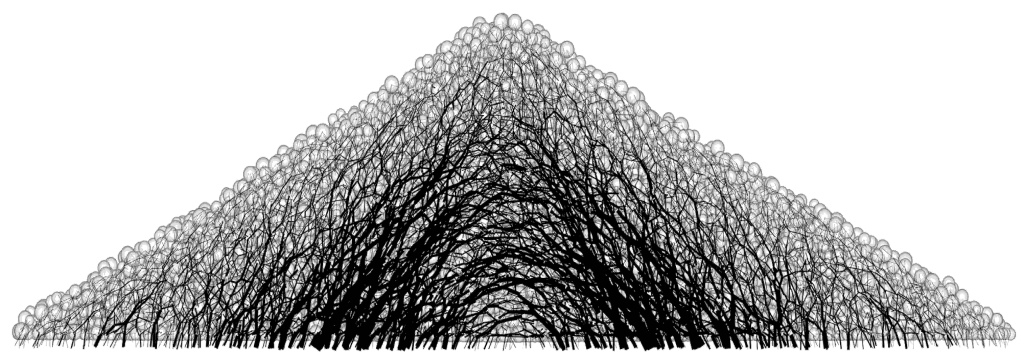
\includegraphics[width=0.9\textwidth]{force_chains.jpg}
    \caption{Силовая сеть в гранулированной насыпи}
    \label{fig:chainheap}
\end{figure}

Такое поведение объясняется полидисперсностью данного материала, за счет чего образуются силовые сети. Силовые сети состоят
из частиц внутри гранулированного материала под давлением, которые удерживаются вместе и заклиниваются сетью взаимных сжимающих сил. 
Между этими цепями находятся участки с низким напряжением, зерна которых "защищены" от воздействия вышеперечисленных зерен сводами и арками (рисунок \ref{fig:chainheap}). 
Набор взаимосвязанных силовых цепей известен как силовая сеть. Очевидно то, что такие полидисперсные материалы способны поглощать энергию и рассеивать ее
в дальнейшем, ведь зачастую такие материалы используются в качестве демпфирующих, но каким образом образующиеся силовые сети влияют на процессы поглощения 
и рассеивания энергии, а так же каким образом они формируются изучено еще недостаточно подробно. Изучение преобразования кинетической энергии поступательного
движения во внутреннюю энергию относительного движения в простейшей силовой цепи  представлено в данной работе.

\begin{figure}[h]
    \centering
    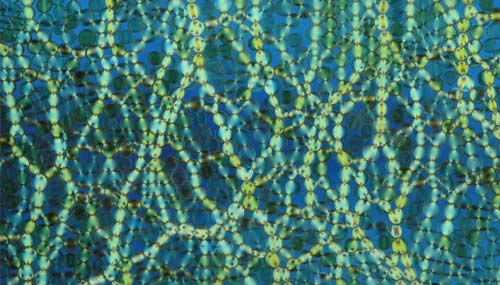
\includegraphics[width=0.9\textwidth]{chains1.jpg}
    \caption{Пример силовой сети полученной при нагружении фотоэластичных гранул}
    \label{fig:chainheap}
\end{figure}